% This work is licensed under the Creative Commons Attribution-NonCommercial 4.0 International License.
% To view a copy of this license, visit http://creativecommons.org/licenses/by-nc/4.0/
% or send a letter to Creative Commons, PO Box 1866, Mountain View, CA 94042, USA.

% !TEX TS-program = xelatex

\documentclass[../Main/chem331-notes.tex]{subfiles}
\begin{document}

\setcounter{section}{10}

\section{The rigid rotor and angular momentum}
\subsection{The classical rigid rotor in 2D}
Consider a particle of mass $m$ that can freely go around a circle of radius $r$ that lays in the $xy$ plane and is perpendicular to the $z$ axis.
The classical Hamiltonian has only one term, the kinetic energy
\begin{equation}
T = \frac{1}{2} m v^2 =  \frac{1}{2} m (v_x^2 + v_y^2).
\end{equation}
In this case it is convenient to work in a polar coordinate system (see Fig.~\ref{fig:rigidrotor:polar}) and use the variables $r$ and $\phi$, which are related to $x$ and $y$ via
\marginpar{
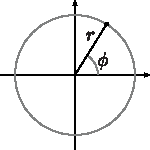
\includegraphics[width=1.0in]{../Figures/RigidRotor/PolarCoordinates.pdf}
\captionof{figure}{Definition of the polar coordinates $r$ and $\phi$.}
\label{fig:rigidrotor:polar}
}
\begin{align}
x & =  r \cos \phi, \\
y & =  r \sin \phi.
\end{align}
Note that in a classical system $r$ is a constant but $\phi$ will be a function of time.
We can also invert these equations and write
\begin{align}
r & =  \sqrt{x^2 + y^2}, \\
\phi & = \arctan\frac{y}{x}.
\end{align}
The components of velocity are given by
\begin{align}
v_x & = \frac{d x}{dt} = - r \sin \phi \frac{d\phi}{dt} = - r \omega \sin \phi , \\
v_y & = \frac{d y}{dt} =   r \cos \phi \frac{d\phi}{dt} =  r \omega \cos \phi,
\end{align}
where we introduced the angular velocity $\omega = \frac{d\phi}{dt}$.
The sum of the squares of the $x$ and $y$ velocity is then given by
\begin{equation}
v^2 = v_x^2 + v_y^2 = r^2 \omega^2 (\sin^2 \phi + \cos^2 \phi ) = r^2 \omega^2,
\end{equation}
and the kinetic energy is given by
\begin{equation}
T = \frac{1}{2} m v^2 =  \frac{1}{2} m r^2 \omega^2 = \frac{1}{2}\frac{\omega^2}{I},
\end{equation}
where $I$ is the \textbf{moment of inertia} defined as
\begin{equation}
I = m r^2.
\end{equation}

Now we want to show that the kinetic energy of the particle on a ring is also related to angular momentum.
Recall that angular momentum is a vector given by the cross product of position and momentum
\begin{equation}
\mathbf{L} = \mathbf{r} \times \mathbf{p}   = m  \mathbf{r} \times \mathbf{v}.
\end{equation}
For a rotating molecule $\mathbf{r}$ and $\mathbf{p}$ are perpendicular, so that $\mathbf{r} \times \mathbf{p}$ has magnitude equal to $m r v$ and will point in the $z$ direction.
Using the fact that $v = r \omega$ we can write the angular momentum in the $z$ direction as
\begin{equation}
L_z = mrv = m r^2 \omega = I \omega.
\end{equation}
Once again we are able to relate all quantities back to $I$ and $\omega$.
From this equation we derive that $\omega = L_z / I$, and substituting this result in the expression for the kinetic energy we get
\begin{equation}
T = \frac{1}{2} I \omega^2 = \frac{1}{2} I \frac{L_z^2}{I^2} = \frac{L_z^2}{2 I}.
\end{equation}
This equation expresses the kinetic energy only in terms of the $z$ component of angular momentum squared $L_z^2$ and the moment of inertia.
Note that since the angular momentum vector has no $x$ and $y$ components, the total angular momentum squared is equal to $L^2 = \mathbf{L} \cdot \mathbf{L} = L_z^2$, and we can write the kinetic energy in terms of $L^2$. 

\subsection{The quantum mechanical rigid rotor in 2D}
Let us now move to work out the quantum mechanics of the rigid rotor.
Our results for the classical particle has important consequences for the quantum mechanical version of this model.
The Hamiltonian will also contain only the kinetic energy term, and in this case we have to impose that the particle distance from the center is a constant
\begin{equation}
\hat{T} = -\frac{\hbar^2}{2 m} \left. \nabla^2 \right|_{r}.
\end{equation}
Again, working in polar coordinates is mandatory.
The derivation of the Laplacian ($\nabla^2$) is a bit involved, but the end result is rather compact.
The Laplacian applied to a function $f$ is given by
%Let us work out the Laplacian
%\begin{equation}
%\frac{\partial}{\partial x} = \frac{\partial r}{\partial x} \frac{\partial}{\partial r} + \frac{\partial\phi}{\partial x} \frac{\partial}{\partial\phi}
%= \cos \phi \frac{\partial}{\partial r} -\frac{1}{r \sin \phi} \frac{\partial}{\partial \phi}
%\end{equation}
%\begin{equation}
%\frac{\partial}{\partial y} = \frac{\partial r}{\partial y} \frac{\partial}{\partial r} + \frac{\partial\phi}{\partial y} \frac{\partial}{\partial\phi}
%= \sin \phi \frac{\partial}{\partial r} +\frac{1}{r \cos \phi} \frac{\partial}{\partial \phi}
%\end{equation}
%and
\begin{equation}
\left(\frac{\partial^2}{\partial x^2} + \frac{\partial^2}{\partial y^2} \right) f
= \frac{1}{r} \frac{\partial}{\partial r} \left( r \frac{\partial f}{\partial r} \right)
+ \frac{1}{r^2} \frac{\partial^2}{\partial \phi^2} f.
\end{equation}
In our case $r$ is a constant and so only the second term in the Laplacian survives.
This means that we can write the Hamiltonian as
\begin{equation}
\label{eq:rigidrotor:hamiltonian_ring}
\hat{H} = -\frac{\hbar^2}{2 m r^2} \frac{\partial^2}{\partial \phi^2}
= -\frac{\hbar^2}{2 I} \frac{\partial^2}{\partial \phi^2}.
\end{equation}
We could go even further and introduce a quantum mechanical operator for angular momentum
\begin{equation}
\hat{\mathbf{L}} = \hat{\mathbf{r}} \times \hat{\mathbf{p}}
\end{equation}
and rewrite the classical energy expression in terms of this operator as
\begin{equation}
\label{eq:rigidrotor:hamiltonian_ring_l2}
\hat{H} =\frac{\hat{L}^2}{2 I},
\end{equation}
where $\hat{L}^2$ is the total angular momentum operator squared
\begin{equation}
\hat{L}^2 = \hat{\mathbf{L}} \cdot \hat{\mathbf{L}} = \hat{L}_x^2 + \hat{L}_y^2 + \hat{L}_z^2.
\end{equation}
Comparing Eq.~\eqref{eq:rigidrotor:hamiltonian_ring} to Eq.~\eqref{eq:rigidrotor:hamiltonian_ring_l2} allows us to identify the angular momentum operators as
\begin{equation}
\hat{L}^2 = -\hbar^2 \frac{\partial^2}{\partial \phi^2}.
\end{equation}

The eigefunctions of the Hamiltonian for a particle on a ring are given by
\begin{equation}
\psi_m(\phi) = A e^{i m \phi}.
\end{equation}
If we apply the Hamiltonian to this expression we see that
\begin{equation}
\hat{H} \psi(\phi) = -\frac{\hbar^2}{2 I} \frac{\partial^2}{\partial \phi^2} A e^{i m \phi}
=\frac{\hbar^2 m^2}{2 I}  A e^{i m \phi},
\end{equation}
which shows that the corresponding eigenvalue is 
\begin{equation}
E_m = \frac{\hbar^2 m^2}{2 I}.
\end{equation}
To find the allowed values of $m$ we impose periodic boundary conditions
\begin{equation}
\psi_m(\phi) = \psi_m(\phi + 2\pi) \Rightarrow  A e^{i m \phi} =  A e^{i m (\phi + 2\pi)}  \Rightarrow  1 =  A e^{i m 2\pi}.
\end{equation}
The last condition can be satisfied if $ m 2\pi$ is a multiple of $2\pi$, which means that $m$ must be an integer.
Therefore, the allowed values of $m$ for a particle on a ring are
\begin{iequation}
m = 0, \pm1, \pm2, \ldots .
\end{iequation}

Lastly, we normalize the wave function in the following way
\begin{equation}
\int_0^{2\pi} |\psi_m(\phi)|^2 \, d\phi = 2 \pi |A|^2 = 1,
\end{equation}
so that
\begin{equation}
\psi_m(\phi) = \frac{1}{\sqrt{2\pi}} e^{i m \phi}.
\end{equation}

\subsection{Spherical coordinates}
Spherical coordinates are the natural set of coordinates to solve problems that reflect some aspect of spherical symmetry.
Spherical coordinates are a triplet of values $(r,\theta,\phi)$ that specify the position of a point in Cartesian coordinates $(x,y,z)$, as illustrated in Fig.~\ref{fig:rigidrotor:spherical}.
\marginpar{
\includegraphics[width=1.5in]{../Figures/RigidRotor/SphericalCoordinates.pdf}
\captionof{figure}{Definition of the spherical coordinates $r$, $\theta$, and $\phi$.}
\label{fig:rigidrotor:spherical}
}
Given the coordinate $(r,\theta,\phi)$ the corresponding point $(x,y,z)$ is given by
\begin{align}
x & =  r \sin \theta \cos \phi, \\
y & =  r \sin \theta \sin \phi, \\
z & =  r \cos \theta.
\end{align}
Note that $\theta$ is the angle with respect to the $z$ axis while $\phi$ is the angle that a point projected onto the $xy$ plane makes with the $x$ axis.
The allowed range for these variables is
\begin{align}
0 \leq & r \leq \infty, \\
0 \leq  & \theta \leq \pi, \\
0 \leq  & \phi \leq 2 \pi.
\end{align}
One can also back transform a Cartesian point $(x,y,z)$ to spherical coordinates
\begin{align}
r & =  \sqrt{x^2 + y^2 + z^2}, \\
\cos \theta & = \frac{z}{r}, \\
\tan \phi & = \frac{y}{x}.
\end{align}

It is also important to learn how to compute integrals in spherical coordinates.
The volume element in 3D space $dx \, dy \, dz$ in spherical coordinates becomes
\begin{equation}
dx \, dy \, dz \rightarrow  r^2 \sin \theta \, dr \, d\theta \, d\phi.
\end{equation}
The quantity $r^2 \sin \theta$ is called the Jacobian determinant (or simply the Jacobian) and accounts for the fact that in spherical coordinates the volume element must be shrinked or expanded depending on the position of the point.
This means that a full integral over all space is computed as
\begin{equation}
\int_{-\infty}^{\infty} dx
\int_{-\infty}^{\infty} dy
\int_{-\infty}^{\infty} dz f(x,y,z) = 
\int_{0}^{\infty} dr
\int_{0}^{\pi} d\theta
\int_{0}^{2\pi} d\phi \,r^2 \sin \theta f(r,\theta,\phi).
\end{equation}

The Laplacian in spherical coordinates is
\begin{equation}
\left(\frac{\partial^2}{\partial x^2} + \frac{\partial^2}{\partial y^2} + \frac{\partial^2}{\partial z^2} \right) f
= \frac{1}{r^2} \frac{\partial}{\partial r} \left( r^2 \frac{\partial f}{\partial r} \right)
+ \frac{1}{r^2 \sin \theta} \frac{\partial}{\partial \theta} \left( \sin\theta \frac{\partial f}{\partial \theta} \right)
+ \frac{1}{r^2 \sin^2 \theta} \frac{\partial^2}{\partial \phi^2} f.
\end{equation}

\subsection{The quantum mechanical rigid rotor in 3D}
The Hamiltonian for a particle moving on a sphere is also just a kinetic energy term with the constraint that the radius is constant
\begin{equation}
\hat{H} = \frac{-\hbar^2}{2m} \left. \nabla^2 \right|_{r}
=   \frac{-\hbar^2}{2m r^2} \left[\frac{1}{ \sin \theta} \frac{\partial}{\partial \theta} \left( \sin\theta \frac{\partial }{\partial \theta} \right)
+ \frac{1}{ \sin^2 \theta} \frac{\partial^2}{\partial \phi^2} \right].
\end{equation}
The eigenfunctions of this Hamiltonian are called \textbf{spherical harmonics} and are commonly indicated with the symbol $Y(\theta,\phi)$.
The spherical harmonics can be written as a product of two functions $ \Theta(\theta)$ and $\Phi(\phi)$ that depend on two quantum numbers $l$ and $m$
\begin{equation}
\psi(\theta,\phi) = Y_{l}^{m}(\theta,\phi) = \Theta_{l}^{m}(\theta) \Phi_m(\phi).
\end{equation}
The first quantum number, $l$ can take any integer value 
\begin{iequation}
l  = 0, 1, 2, \ldots,
\end{iequation}
while the absolute value of $m$ must be less than or equal to $l$, $|m| \leq l$, so that
\begin{iequation}
\label{eq:rigidrotor:m}
m  = 0, \pm1, \pm2, \ldots, \pm l.
\end{iequation}

The spherical harmonics are eigenfunctions of the particle on a sphere Hamiltonian and their eigenvalues depend only on the quantum number $l$
\begin{iequation}
\hat{H}  Y_{l}^{m}(\theta,\phi) = \frac{\hbar^2 l(l+1)}{2m r^2}  Y_{l}^{m}(\theta,\phi).
\end{iequation}
Since for one value of $l$ we can have $2l +1$ values of $m$ [counting all possible values according to Eq.~{eq:rigidrotor:m}], the degeneracy of each level with fixed $l$ is $g_l = 2l +1$.

The $\phi$-dependent part of spherical harmonics is the same as the wave function of a particle on a ring
\begin{equation}
\Phi_m(\phi) = \frac{1}{\sqrt{2\pi}}e^{im\phi}.
\end{equation}
The $\theta$-dependent term $\Theta_{l}^{m}(\theta)$ is given by
\begin{equation}
\Theta_{l}^{m}(\theta) = \left[ \frac{2l +1}{2} \frac{(l - |m|)!}{(l + |m|)!} \right]^{1/2} P_l^{|m|}(\cos\theta),
\end{equation}
where $P_l^m(x)$ is an \textbf{associated Legendre polynomial}.
Here are some of the low order polynomials as a function of $x = \cos \theta$
\begin{equation}
\begin{split}
P_0^0(x) & = 1, \\
P_1^0(x) & = x = \cos \theta, \\
P_1^1(x) & = \sqrt{1 - x^2} = \sin \theta, \\
P_2^0(x) & = \frac{1}{2} (3x^2 -1) = \frac{1}{2}(3\cos^2 \theta - 1), \\
P_2^1(x) & = 3x\sqrt{1 - x^2} = 3\cos \theta \sin \theta, \\
P_2^2(x) & = 3(1 - x^2) = 3\sin^2 \theta.
\end{split}
\end{equation}

When combined together, the low order spherical harmonics are given by
\begin{equation}
\begin{split}
Y_0^0(\theta,\phi) & = \left( \frac{1}{4\pi} \right)^{1/2},  \\
Y_1^0(\theta,\phi) & = \left( \frac{3}{4\pi} \right)^{1/2} \cos \theta,  \\
Y_1^{\pm1}(\theta,\phi) & = \left( \frac{3}{8\pi} \right)^{1/2} \sin \theta e^{\pm i\phi}, \\
Y_2^0(\theta,\phi) & = \left( \frac{5}{16\pi} \right)^{1/2} (3\cos^2 \theta - 1), \\
Y_2^{\pm1}(\theta,\phi) & = \left( \frac{15}{8\pi} \right)^{1/2} \cos \theta \sin \theta e^{\pm i\phi}, \\
Y_2^{\pm2}(\theta,\phi) & = \left( \frac{15}{32\pi} \right)^{1/2} \sin^2 \theta e^{\pm 2i\phi}.
\end{split}
\end{equation}

\subsection{Properties of spherical harmonics}
The spherical harmonics satisfy some important properties.
First, they are orthonormalized, so that an integral in the following sense
\begin{iequation}
\int_{0}^{\pi} d\theta
\int_{0}^{2\pi} d\phi \, \sin \theta \, Y_l^{m}(\theta,\phi)^*   Y_{l'}^{m'}(\theta,\phi) = \delta_{l,l'} \delta_{m,m'} .
\end{iequation}
That is, this integral is one only if both $l = l'$ and $m = m'$.

It is also possible to show that spherical harmonics are eigenfunctions of the angular momentum operator squared 
\begin{iequation}
\hat{L}^2 Y_l^{m}(\theta,\phi) = \hbar^2 l(l+1) Y_l^{m}(\theta,\phi),
\end{iequation}
which illuminates the meaning of the quantum number $l$. This number determines the total value of angular momentum (how much the system spins in space) and controls also the total energy of the particle on a sphere.
Spherical harmonics are also eigenfunctions of the $z$-projection of the angular momentum operator
\begin{iequation}
\hat{L}_z Y_l^{m}(\theta,\phi) = \hbar m Y_l^{m}(\theta,\phi).
\end{iequation}
Hence, $m$ determines the projection of momentum onto the $z$ axis.

\subsection{Rotation in diatomic molecules}
Consider a diatomic molecule with atoms of mass $m_1$ and $m_2$ and a \textbf{fixed} bond distance $r$.
We assume that the center of mass coincides with the origin and that the distance of the first and second atom from the origin is equal to $r_1$ and $r_2$, respectively, as shown in Fig.~\ref{fig:rigidrotor:rigidrotor}.
\marginpar{
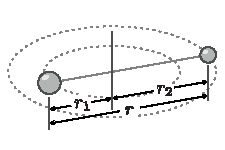
\includegraphics[width=1.5in]{../Figures/RigidRotor/RigidRotor.pdf}
\captionof{figure}{Definition of the quantities $r_1$, $r_2$, and $r = r_1 + r_2$ for the rigid rotor model.}
\label{fig:rigidrotor:rigidrotor}
}
%\mnote{
%\begin{tikzpicture}
%%  \draw (0,0) circle (1cm);
%  \draw[<->] (-0.5,0) -- (1.,0) node[above] {$r_1$};
%  \draw[<->] (-1.0,0) -- (-0.5,0) node[above] {$r_2$};
%\end{tikzpicture}
%}
The classical kinetic energy is given by
\begin{equation}
T = \frac{1}{2} m_1 v_1^2 + \frac{1}{2} m_2 v_2^2,
\end{equation}
where $v_1$ and $v_2$ are the radial velocities of atoms 1 and 2.
We can relate the radial velocity to the angular velocity $\omega$ via
\begin{align}
v_1 = \omega r_1 \\
v_2 = \omega r_2.
\end{align}
This allows us to write the kinetic energy in terms of the angular velocity $\omega$
\begin{equation}
T = \frac{1}{2} m_1 \omega^2 r_1^2 + \frac{1}{2} m_2 \omega^2 r_1^2
 = \frac{1}{2} (m_1 r_1^2 + m_2 r_1^2)  \omega^2 
 = \frac{1}{2} I \omega^2.
\end{equation}
The quantity $I$ is called the \textbf{moment of inertia}\mnote{The fact that the moment of inertia depends on the bond length $r$ suggests that spectroscopies that measure rotational energy levels can potentially provide geometric information about molecules. This is indeed the case.} 
The moment of inertia is
\begin{equation}
I = m_1 r_1^2 + m_2 r_2^2. % = \mu r^2.
\end{equation}
To simplify this expression consider the molecule aligned along the $x$ axis and let us assume that the center of mass $r = (m_1 r_1 - m_2 r_2)/ M$ is centered at the origin, that is, $r = 0$. It follows that $m_1 r_1 = m_2 r_2$.
Using the fact that $r = r_1 + r_2$, we can derive expressions for $r_1$ and $r_2$ in terms of $r$
\begin{equation}
m_1 r_1 = m_2 (r - r_1) \Rightarrow r_1 = r \frac{m_2}{M},
\end{equation}
and
\begin{equation}
m_2 r_2 = m_1 (r - r_2) \Rightarrow r_2 = r \frac{m_1}{M}.
\end{equation}
From which follows that
\begin{iequation}
I = m_1 r_1^2 + m_2 r_2^2 = m_1 r^2 \frac{m_2^2}{M^2} + m_2 r^2 \frac{m_1^2}{M^2}
 = \frac{m_1 m_2 (m_1 + m_2)}{M^2}  r^2 = \mu r^2,
\end{iequation}
where $\mu$ is the reduced mass that we encountered already when we studied the vibrations of a diatomic molecule.
Note that this is the same expression we would have derived if we considered \textbf{a single particle} of mass $\mu$ rotating around the origin at a fixed distance $r$.
Hence for a molecule rotating in 3D the energy expression is
\begin{equation}
E_l = \frac{\hbar^2 l(l+1)}{2 \mu r^2} = \frac{\hbar^2  l(l+1)}{2 I}, 
\end{equation}
that is, we have to modify our definition of moment of inertia to use the reduced mass and the bond length as the radius.

\end{document}





